\documentclass[10pt,a4paper]{article}
\usepackage[latin1]{inputenc}
\usepackage{amsmath}
\usepackage{microtype}
\usepackage[none]{hyphenat}
\usepackage{verbatim}
\usepackage{amsfonts}
\usepackage{amssymb}
\usepackage{enumitem}
\renewcommand{\familydefault}{\sfdefault}
\usepackage{mathpazo}
\renewcommand{\rmdefault}{put}
\usepackage{enumitem}
\usepackage[dvipsnames,svgnames]{xcolor}
\usepackage{tkz-euclide}
\usetkzobj{all}
\usepackage{graphicx}
\usetikzlibrary{calc,patterns,angles,quotes}
\usepackage{tikz} 	
\usepackage{adjustbox}
\usepackage{multicol}
\usepackage{lipsum}
\usepackage[left=0.1cm,right=0.7cm,top=0.2cm,bottom=1.5cm]{geometry}
\usepackage{cancel} \usepackage{xcolor}
\usepackage{tcolorbox}
\usetikzlibrary{decorations.pathmorphing,patterns,shapes.geometric}
\usetikzlibrary{decorations.pathreplacing,calc}
 \newcommand\coret[2][red]{\renewcommand\CancelColor{\color{#1}}\cancel{#2}}

%%_------= solusi


% Set this =0 to hide, =1 to show

% Set this =0 to hide, =1 to show
\newtcolorbox{mybox}[1][] { colframe = blue!10, colback = blue!3,boxsep=0pt,left=0.2em, coltitle = blue!20!black, title = \textbf{jawab}, #1, } 


\def\showanswers{1}
\newcommand{\hide}[1]{\ifnum\showanswers=1
%
\begin{mybox}
 #1
\end{mybox}
%
\vspace{\baselineskip}\fi\ifnum\showanswers=0\vspace{2\baselineskip} \hspace{2cm}\fi}



\newcommand*\cicled[1]{\tikz[baseline=(char.base)]{\node[white, shape=circle, fill=red!80,draw,inner sep=0.5pt](char){#1};}}

\newcommand*\lingkaran[1]{\tikz[baseline=(char.base)]{\node[red, shape=circle,draw,inner sep=0.5pt](char){#1};}\stepcounter{enumii}}

\newcommand*\silang[1]{\tikz[baseline=(char.base)]{
\draw[red,thick](-0.2,-0.20)--(0.2,0.2);
\draw[red,thick](-0.2,0.20)--(0.2,-0.2);
\node[black](char){#1};
}}


\newcommand*\centang[1]{\tikz[baseline=(char.base)]{
\draw[red, very thick](-0.2,0.1)--(-0.1,0)--(0.2,0.3);
\node(char){#1};
}}

\newcommand*\merah[1]{
\textcolor{red}{#1}}
\newcommand*\pilgan[1]{
\begin{enumerate}[label=\Alph*., itemsep=0pt,topsep=0pt,leftmargin=*] #1 
\end{enumerate}}
\newcommand*\pernyataan[1]{
\begin{enumerate}[label=(\arabic*), itemsep=0pt,topsep=0pt,leftmargin=*] #1 
\end{enumerate}}



\begin{document}

\setlength{\abovedisplayskip}{0pt}
\setlength{\belowdisplayskip}{3pt}
\setlength{\abovedisplayshortskip}{0pt}
\setlength{\belowdisplayshortskip}{3pt}
%-----------------------------------------------

 \centering
  \renewcommand{\arraystretch}{2}
  \begin{tabular}{  |>{\centering\arraybackslash}m{4cm}|%
                    >{\centering\arraybackslash}m{11cm}|%
                    >{\centering\arraybackslash}m{4cm}|%
  }
    \hline
    \vspace{0.15cm} 
    \tikz[baseline=(char.base)]{
\draw[green!80!black](-0.3,-0.2) rectangle (0.3,0.2);
\node[green](char){line};
} \small{ arifstwan} &       \textbf{ } 
          & bintangpelajar.com 
  \\ \hline 
    
  \end{tabular}
\setlength{\columnsep}{0.2cm}
\renewcommand{\columnseprulecolor}{\color{blue!40}}

\vspace{0.15cm}

\begin{multicols*} {2} 
 \setlength{\columnseprule}{0.4pt}
\newcommand{\tikzmark}[2]{\tikz[remember picture,baseline=(#1.base)]{\node[inner sep=0pt] (#1) {#2};}} 


\begin{enumerate}[itemsep=0mm]

%A double line with ends are closed - manually created
\item 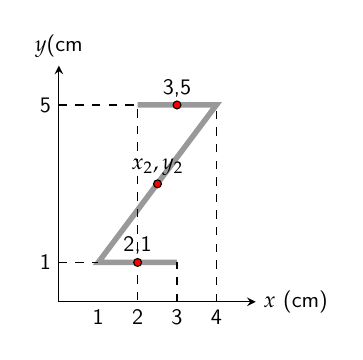
\begin{tikzpicture}[scale=0.5]
\draw[stealth-stealth](0,6) node [above, scale=0.8]{$y$(cm} -- (0,0) -- (5,0)node [right,scale=0.8]{$x$ (cm)};
\draw[line width = 2pt,gray!80 ](3,1)--(1,1)--(4,5)--(2,5);
\draw[dashed](0,1)--(1,1)(0,5)--(2,5)--(2,0)(3,0)--(3,1)(4,0)--(4,5);
\foreach \x in {1,2,3,4}{
\node at (\x,0)[below,scale=0.8]{\x};}
\foreach \y in {1,5}{
\node at (0,\y)[left,scale=0.8]{\y};}
\foreach \x/\y in {2/1,3/5}{\node at (\x,\y)[above, scale=0.8]{\x,\y};
 \draw[fill=red](\x,\y)circle(0.1cm);
}
\node at ($(1,1)+(53:2.5)$)[above,scale=0.8]{$x_2,y_2$};
\draw [fill=red]($(1,1)+(53:2.5)$)circle(0.1cm);
\end{tikzpicture}

Untuk menghitung tinggi $x_2$ dan $y_2$ perlu digambar segitiga

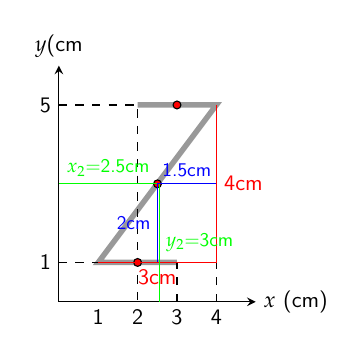
\begin{tikzpicture}[scale=0.5]
\draw[stealth-stealth](0,6) node [above, scale=0.8]{$y$(cm} -- (0,0) -- (5,0)node [right,scale=0.8]{$x$ (cm)};
\draw[line width = 2pt,gray!80 ](3,1)--(1,1)--(4,5)--(2,5);
\draw[dashed](0,1)--(1,1)(0,5)--(2,5)--(2,0)(3,0)--(3,1)(4,0)--(4,5);
\foreach \x in {1,2,3,4}{
\node at (\x,0)[below,scale=0.8]{\x};}
\foreach \y in {1,5}{
\node at (0,\y)[left,scale=0.8]{\y};}
\foreach \x/\y in {2/1,3/5}{
 \draw[fill=red](\x,\y)circle(0.1cm);
}
\draw [fill=red]($(1,1)+(53:2.5)$)circle(0.1cm);
\draw[red](1,1)--node[below,midway,scale=0.8]{3cm}(4,1)--node[right,midway,scale=0.8]{4cm}(4,5);
\draw[blue](2.5,3)--node[left,midway,scale=0.7]{2cm}(2.5,1);
\draw[blue](2.5,3)--node[above,midway,scale=0.7]{1.5cm}(4,3);
\draw[green](2.55,3)--node[right,midway,scale=0.7]{$y_2$=3cm}(2.55,0);
\draw[green](2.5,3.01)--node[above,midway,scale=0.7]{$x_2$=2.5cm}(0,3.01);
\end{tikzpicture}
\hide{
Untuk mengerjakan perhatikan $L$ adalah panjang masing-masing ruas, dan garis warna hijau adalah posisi titik berat garis miring. Panjang garis miring adalah 5 cm berdasarkan gambar tersebut (phytagoras)
\\
\begin{align*}
x&=\frac{x_1L_1+x_2L_2+x_3L_3}{L_1+L_2+L_3}\\
x&=\frac{(2)(2)+(2.5)(5)+(3)(2)}{2+5+2}\\
x&=\frac{22,5}{9}=\frac{45}{18}=2,5 \text{ cm}
\end{align*}
\begin{align*}
y&=\frac{y_1L_1+y_2L_2+y_3L_3}{L_1+L_2+L_3}\\
y&=\frac{(1)(2)+(3)(5)+(5)(2)}{2+5+2}\\
y&=\frac{27}{9}=3 \text{ cm}
\end{align*}}
\vspace{7cm}

\item $T=2\pi \sqrt{\frac{m}{k}}$ untuk menentukan $k$ degan rumus
\begin{align*}
T&= 2\pi \sqrt{\frac{m}{k}}\\
T^2&=4\pi^2\frac{m}{k}\\
k&=4\pi^2\frac{m}{T^2}
\end{align*}
Lah buat menentukan ketidakpastiannya menggunakan rumus gayut
$$f(x,y,z)$$
$$\Delta f = \frac{\partial f}{\partial x}\Delta x + \frac{\partial f}{\partial y}\Delta y +\frac{\partial f}{\partial z}\Delta z$$
Maka persamaannya diubah menjadi 
\\
\begin{align*}
k&=4\pi^2.m.T^{-2}
\end {align*}
\begin{align*}
\Delta k &= |\frac{\partial k}{\partial m} \Delta m| +|\frac{\partial k}{\partial T}\Delta T|\\
\Delta k &= |\frac{\partial m.T^{-2}}{\partial m}\Delta m|+|\frac{\partial m.T^{-2}}{\partial T}\Delta T|\\
\Delta k &=| T^{-2}\Delta m| +|-2.m.T^{-3}\Delta T|
\end{align*}

a. ketidak pastian relatif = $\frac{\Delta k}{k}$\\
b. Ketidak pastian (masukin aja angka persamaan $\Delta k$ tersebut


\end{enumerate}
\end{multicols*}
\end{document}

%--------------------- Selesai-------
